\documentclass[twoside]{scrartcl}

\usepackage[blacklinks]{drangreport}
% \usepackage[caecilia]{drangreport}

\usepackage{tikz}
\usepackage{amsfonts}

\usepackage[makeroom]{cancel}
\title{Mechanics}
\def\logo@{\rightline{\eightpoint Typeset by \AmSTeX}}

%Nice end of Proof Symbol
\usepackage{marvosym}
\renewcommand{\qedsymbol}{\Rectsteel} 


\begin{document}


\NotesTitle{1st}{Spring 2015}{Mechanics}{Dr.~E.}{Keaveny}
{
{\Large\bfseries\sffamily{Syllabus}}

\textit{This introductory course on Applied Mathematics is centred on Newtonian mechanics - the consequences of Newton’s laws. Some of the course overlaps with A-level Applied Mathematics. It includes far-reaching ideas on energy, linear and angular momentum, simple oscillatory systems and motion under central forces such as planetary motion.}

\begin{itemize}
\item \textbf{Kinematics of point particles:} Vectors and vector algebra; position, velocity, and acceleration in three dimensions; polar coordinates; intrinsic coordinates and path curvature.
\item \textbf{Kinetics and Newton's laws:} Definition of mass, momentum, inertia, and force; Axioms, or Laws of Motion
\item \textbf{Forces:} Gravitation; forces that constrain motion: normal force and tension; friction; forces that depend on velocity: drag forces; forces that depend on position: spring forces. 
\item \textbf{Oscillators:} Simple, damped, and forced oscillators; amplitude and phase difference; resonance.
\item \textbf{Energy:} Kinetic and potential energies; conservative forces; stability of and motion about fixed points; potential wells and escape; energy diagrams.
\item \textbf{Angular momentum:} Central forces; orbital equation; effective potential.
\item \textbf{Systems of (interacting) particles:} Two body systems; centre of mass; moment of inertia; total momentum, angular momentum, and energy for systems; variable mass systems; torque;
\item \textbf{Rigid body motion:} Rigid body kinematics; continuous mass distributions; rigid body dynamics with rotation about a single axis
\end{itemize}

\subsection*{Appropriate books}

{\shortskip
D.~Kleppner and R.~J.~Kolenkow \emph{An Introduction to Mechanics}.

G.~R.~Fowles and G.~L.~Cassiday \emph{Analytical Mechanics}.

R.~Feynman \emph{The Feynman Lectures}.

T.~W.~B.~Kibble and F.~H.~Berkshire \emph{Classical Mechanics}.

}}

\TableofContents

%!TEX root = linear-algebra.tex
\stepcounter{lecture}
\setcounter{lecture}{1}
\pagebreak
\sektion{Kinematics}


\lecturemarker{1}{5 Oct}

\setcounter{page}{4}

What we are after is an \emph{equation of motion} to find the position of an object for all times. Ingredients to an equation of motion:\begin{enumerate}
\item[1)] Kinematics - Description of motion 
\item[2)] Kinetics - Newton's laws
\item[3)] Mathematical Description of Forces - Describe forces in terms of kinematic quantities
\end{enumerate}


\subsektion{Cartesian Coordinates} % (fold)
\label{sub:sets}



For a point particle there are three key kinematic quantities.\begin{enumerate}
\item[1.] Positon: $\vec{r}(t)$
\item[2.] Velocity: $\vec{v}(t)$
\item[3.] Acceleration: $\vec{a}(t)$

In general, $\vec{r}(t),~\vec{v}(t),~\vec{a}(t) \in \mathbb{R}^3$. 
\end{enumerate}\vspace*{5pt}

We can use different coordinate systems to describe our quantities:
\begin{enumerate}
\item Cartesian
\item Polar
\item Intrinsic	
\end{enumerate}

Consider the path of a particle through space:

\vspace*{100pt}

\begin{definition} We write the \emph{position} at time $t$ as
\[\vec{r}(t) = x(t)\hat{i} + y(t)\hat{j} + z(t)\hat{k}\]
We can also write this as
\[[\vec{r}(t)] = \left[\begin{smallmatrix}
x(t)\\ y(t) \\ z(t)	
\end{smallmatrix}
 \right]\text{ so, } \hat{i} =  \left[\begin{smallmatrix}
1\\0\\0
\end{smallmatrix}
 \right],~ \hat{j} =  \left[\begin{smallmatrix}
0\\j\\0
\end{smallmatrix}
 \right],~ \hat{k} =  \left[\begin{smallmatrix}
0\\0\\1
\end{smallmatrix}
 \right]\]
 \textit{Magnitude of $\vec{r}$} \[r = |\vec{r}| = \sqrt{x^2 + y^2 + z^2}\]
$r$ is the distance from the origin.
 
 \textit{Direction of $\vec{r}$} \[\hat{r} = \vec{r}/r = \frac{x}{r}\hat{i} + \frac{y}{r}\hat{j} + \frac{z}{r}\hat{k}\]
  \end{definition}
  
 So, we can write 
 \[\vec{r} = r(t)\hat{r}(t)\]
 This is the starting point for polar coordinates.\\

  \lecturemarker{2}{5 Oct}
 \textbf{Last Time:}
 \vspace*{100pt}



Position: 
\[\vec{r}(t) = x(t)\hat{i} + y(t)\hat{j} + z(t)\hat{k}\]
At $\Delta t$ later
\[\vec{r}(t + \Delta t) = x(t + \Delta t)\hat{i} + y(t + \Delta t)\hat{j} + z(t + \Delta t)\hat{k}\]

\begin{definition}
Define $\Delta \vec{r} = \vec{r}(t + \Delta t) - \vec{r}(t)$

Define the \emph{velocity} of the particle at time $t$
\[\vec{v}(t) = \lim_{\Delta t \to 0} \frac{\Delta \vec{r}}{\Delta t} = \frac{\mathrm{d}\vec{r}}{\mathrm{d}t}\]
\end{definition}

Since $\hat{i},\hat{j},\hat{k}$ are constant in time
\[\begin{aligned}
	\vec{v}(t) = \frac{\mathrm{d}}{\mathrm{d}t}(\vec{r}(t)) &= \frac{\mathrm{d}}{\mathrm{d}t}(x \hat{i} + y\hat{j} + z\hat{k})\\
	&= \frac{\mathrm{d}x}{\mathrm{d}t}\hat{i} + \frac{\mathrm{d}y}{\mathrm{d}t}\hat{j} + \frac{\mathrm{d}z}{\mathrm{d}t}\hat{k}
\end{aligned}
\]
Writing $\dfrac{\mathrm{d}f}{\mathrm{d}t} \equiv \dot{f}$, \[\vec{v}(t) = \dot{x}\hat{i} + \dot{y}\hat{j} + \dot{z}\hat{k} = v_x\hat{i} + v_y\hat{j} + v_z\hat{k}\]

\begin{definition}
\[v = |\vec{v}| = [v_x^2 + v_y^2 + v_z^2]^{1/2}\]
is the magnitude of the velocity or \emph{speed} of the particle.

Thus, the \emph{direction} of motion is 
\[\hat{v} = \vec{v}/v,~ |\hat{v}| = 1\]
$\hat{v}$ is also the unit tangent to the path.

Define the \emph{acceleration}
\[\vec{a}(t) = \frac{d\vec{v}}{dt} = \frac{d^2\vec{r}}{dt^2} = \ddot{x}\hat{i} + \ddot{y}\hat{j} + \ddot{z}\hat{k}\]
\end{definition}

$\vec{a}(t)$ tells us how the velocity is changing at time $t$. 

Recall that we can write 
\[\vec{v} = v(t)\hat{v}(t), \text{ then } \vec{a} = \]

\subsektion{Polar Coodinates}
\pagebreak


\subsektion{Intrinsic Coordinates}

\lecturemarker{7}{5 Oct}

Coordinates that are intrinsic to the path of our particle. We know the path!
\vspace*{120pt}

Distance travelled between $t$ and $t + \Delta t$
:
\[\Delta s = |\Delta \vec{r}| = \left|[x(t + \Delta t) - x(t)]\hat{i} + [y(t + \Delta t) - y(t)]\hat{j} + [z(t + \Delta t) - z(t)]\hat{k}\right|\]
For $\Delta t << 1$: 
\[x(t + \Delta t) = x(t) + \Delta t \frac{dx}{dt} + \cal{O}(\Delta t^2)\]
Doing the same for our other components:
\[\Delta s = \underbrace{\left|\frac{dx}{dt}\hat{i} + \frac{dy}{dt}\hat{j} + \frac{dz}{dt}\hat{k}\right|}_{\vec{v}}\Delta t + \cal{O}(\Delta t^2)\]

Thus,
\[\frac{\Delta s}{\Delta t} = v + \cal{O}(\Delta t)\]
Taking $\lim \Delta t \to 0$
\[\boxed{\frac{ds}{dt} = v = \dot{s} \implies s(t) = \int_0^t v(t')\,dt'}\]
Both $t$ and $s$ are ways of parametrizing our curve (path). Instead of writing $\vec{r}(t)$, we can write $\vec{r}(s)$. \\

\begin{definition} $s$ is what we call the \emph{arc length}. 

$\displaystyle{\vec{v} = \frac{d\vec{r}}{dt} = \frac{d\vec{r}}{ds}\frac{ds}{dt}}$. But $\displaystyle{\frac{ds}{dt} = v}$. So, $\displaystyle{\frac{d\vec{r}}{ds} = \hat{v}}$, the unit tangent at evert point $s$. Thus
\[\vec{v}(s) = \dot{s}\hat{v}\]

Also \[\begin{aligned}
	\vec{a} = \frac{d\vec{v}}{dt} = \frac{d}{dt}\left(\dot{s}~ \frac{d\vec{r}}{ds}\right) = \ddot{s}\frac{\d\vec{r}}{ds} + \dot{s}\frac{d}{dt}\left(\frac{d\vec{r}}{ds}\right) &= \ddot{s}\hat{v} + \dot{s}\frac{d^2\vec{r}}{ds^2}\frac{ds}{dt}
\end{aligned}
\]

So
\[\vec{a}(s) = \ddot{s}\hat{v} + \dot{s}^2\frac{d^2\vec{r}}{ds^2} = \ddot{s}\hat{v} + \kappa \dot{s}^2\hat{n}\]
Writing $\displaystyle{\frac{d^2\vec{r}}{ds^2} = \kappa \hat{n}}$, where $\displaystyle{\kappa =\left|\frac{d^2\vec{r}}{ds^2}\right| }$, $\hat{n} = \displaystyle{\frac{1}{\kappa}\frac{d^2\vec{r}}{ds^2}}$.
\end{definition}

It turns out that $\kappa$ is the curvature of the path. What about $\hat{n}$?

Recall: $|\hat{v}| = 1$. So $\frac{d}{ds}(\hat{v}\cdot\hat{v} = 1) \implies 2\hat{v}\cdot\frac{d\hat{v}}{ds} = 0 \implies 2\kappa(\hat{v}\cdot\hat{n}) = 0$

So, if $\kappa \neq 0$, then $\hat{v}\cdot \hat{n} = 0$. Thus $\hat{n}$ is the unit normal to the path.\\

Tangential component of the acceleration $a_t = \vec{a}\cdot\hat{v} = \ddot{s}$

Normal component of the acceleration $a_n = \vec{a}\cdot\hat{n} = \kappa \dot{s}^2$, where $\kappa \approx 1/R$
\vspace*{100pt}

Key things to note: $\hat{v}, \hat{n}, \kappa$ depend only on the path. Knowing $\vec{r}(s)$, we can find these 	quantities. 

$\dot{s}$ and $\ddot{s}$ depend on how the particle is moving along the path.\\


\begin{example}[Circular Motion]~\\

\textbf{Cartesian:}
$\vec{r}(t) = R\sin(\omega t)\hat{i} + R\cos(\omega t)\hat{j}$.
Differentiating finds $\vec{v}(t)$ and $\vec{a}(t)$.\\

\textbf{Polars:} 
$r = R$ and $\theta = \frac{\pi}{2} \omega t \implies \dot{r} = \ddot{r} = 0$ and $ \dot{\theta} = -\omega,~\ddot{\theta} = 0$. So 

\[\begin{aligned}
	\vec{r} &= R\hat{r}\\
 \vec{v} &= \dot{r}\hat{r} + r\dot{\theta}\hat{\theta} = -R\omega\hat{\theta}\\
\vec{a} &= (\ddot{r} - r\dot{\theta}^2)\hat{r} + (2\dot{r}\dot{\theta} + r\ddot{\theta})\hat{\theta} = -R\omega^2\hat{r}
\end{aligned}
\]~

\textbf{Intrinsic:} ($s(0) = 0$) The speed is given by $v = R\omega = \dot{s} \implies \ddot{s} = 0$. Integrate to find $s$
\[s = R\omega t \implies t= \frac{s}{R\omega}\]
Substitute this into our expression for $\vec{r}(t)$
\[\vec{r}(s) = R\sin(s/R)\hat{i} + R\cos(s/R)\hat{j}\]

$\implies \hat{v} = \dfrac{d\vec{r}}{ds} = \cos(s/R)\hat{i} - \sin(s/R)\hat{j}$,
$~~\dfrac{d^2\vec{r}}{ds^2} = -\dfrac{1}{R}[\sin(s/R)\hat{i} + \cos(s/R)\hat{j}]$

$\implies \kappa = \left|\dfrac{d^2\vec{r}}{ds^2} \right| = \dfrac{1}{R}$, $\hat{n} = -\sin(s/R)\hat{i} - \cos(s/R)\hat{j}$

\[\begin{aligned}
\vec{v}(s) &= R\omega \hat{v}\\
\vec{a}(s) &= \ddot{s}\hat{v} + \kappa \dot{s}^2\hat{n} = \frac{1}{R}(R\omega)^2\hat{n} = R\omega^2\hat{n}
\end{aligned}
\]
\end{example}


\begin{example}[Helical Path]\lecturemarker{8}{5 Oct}
	\[\vec{r}(s) = b\cos(ks)\hat{i} + b\sin(ks)\hat{j} + s\sqrt{1-b^2k^2}\hat{k}\]
	
	Tangent:
	\[\vec{v} = \frac{d\vec{r}}{ds} = -bk\sin(ks)\hat{i} + bk\cos(ks)\hat{j} + \sqrt{1-b^2k^2}\hat{k}\]~
	
	Curvature and Normal:
	\[\frac{d^2\vec{r}}{ds^2} = -bk^2\cos(ks)\hat{i} -bk^2 \sin(ks)\hat{j}\]
	\[\kappa =\left|\frac{d^2\vec{r}}{ds^2}\right| = bk^2,~ \hat{n} =  -\cos(ks)\hat{i} -\sin(ks)\hat{j}\]
	
Take $s = ct$ ($c >0$) $ \implies \dot{s} =c,~ \ddot{s} = 0$. Thus
\[\vec{v} = c\hat{v},~\vec{a} = c^2bk^2\hat{n}\]	
\end{example}

Take the case where our path lies in the $xy-$plane and we know $y(x)$
\vspace*{100pt}

Then $ds^2 = dx^2 + dy^2$. Since $dy = \frac{dy}{dx}dx \implies ds^2 = (1 + (\frac{dy}{dx})^2 )dx^2$
\[\implies \frac{ds}{dx} = \sqrt{1 + y'^2}\]
\[s(x) = \int_{x_0}^x (1 + y'^2)^{1/2}dx\]

Highlights that $s$ just depends on the path. 


Position $\vec{r}(x) = x\hat{i} + y(x)\hat{j}$

Tangent to the path
\[\hat{v} = \frac{d\vec{r}}{ds} = \frac{d\vec{r}}{dx}\frac{dx}{ds} = \frac{d\vec{r}}{dx}\left(\frac{ds}{dx}\right)^{-1}\]
\[\frac{d\vec{r}}{dx} = \hat{i} + y'\hat{j},~~\left(\frac{ds}{dx}\right)^{-1} = [1 + y'^2]^{-1/2}\]
\[\implies \hat{v} = [1+y'2]^{-1/2}[\hat{i} + y'\hat{j}]\]

Curvature and Normal
\[\frac{d^2\vec{r}}{ds^2} = \frac{d}{dx}\left(\frac{d\vec{r}}{ds}\right)\left(\frac{ds}{dx}\right)^{-1} = \left(\frac{d}{dx}\left(\frac{d\vec{r}}{ds}\right)\frac{dx}{ds}\right)\]
\[\frac{d}{dx}\frac{d\vec{r}}{ds} = \frac{d\hat{v}}{dx} = -\frac{1}{2}[1+y'^2]^{-3/2} \times (2y'y'')\times [\hat{i} + y'\hat{j}] + [1 + y'^2]^{-1/2}y''\hat{j}\]~


\begin{example}
$y = x^2,~y' = 2x,~ y'' = 2$

\[\frac{ds}{dx} = [1 + y'^2]^{1/2}\]	
\end{example}








		% Vector spaces
%!TEX root = linear-algebra.tex
\stepcounter{lecture}
\setcounter{lecture}{2}
\sektion{Kinetics and Newtons Laws}
\subsektion{Newton's Laws}
\lecturemarker{9}{22 Oct}
\begin{definition}
\begin{itemize}

\item \emph{Mass, $m$} - ``Quantity of Matter'', measured in kg (scalar)

\item \emph{Momentum, $\vec{p} = m\vec{v}$} - ``Quantity of Motion'' (vector)

\item \emph{Inertia} - ``Vis Insita'' (innate force of matter). The resistance of an object to change its state of motion.

\item \emph{Force} - An action that changes an objects state of motion
\end{itemize}
\end{definition}

\begin{theorem}[Newton's First Law]
Every body has inertia. 	
\end{theorem}


\begin{theorem}[Newton's Second Law]
The net force on an object is equal to the rate of change of momentum:

\[ \vec{F} = \frac{d\vec{p}}{dt} = \frac{d(m\vec{v})}{dt}\]
\end{theorem}

\begin{theorem}[Newton's Third Law]
If $\vec{F}_{AB}$ is the force on object $A$ due to object $B$. Then $\vec{F}_{BA} = -\vec{F}_{AB}$.
\end{theorem}

		% Endomorhisms
%!TEX root = linear-algebra.tex
\stepcounter{lecture}
\setcounter{lecture}{3}

\sektion{Forces}
\subsektion{Gravity}
\subsektion{Contraint Forces}
\subsektion{Friction}
\subsektion{Drag Force}
\lecturemarker{15}{22 Oct}

Example of a force that depends on the velocity of an object. 

Motion of bodies through fluid. 
\vspace*{100pt}

Fluid has: $\rho$: density and $\eta$: viscosity

To move through the fluid, the body exerts a force on the fluid: $\vec{F}_{FB}$

By Newton's III Law
\[\vec{F}_{BF} = -\vec{F}_{FB}\]
The drag force \[\vec{F}_D = (\vec{F}_{BF}\cdot \hat{v})\hat{v}\]

In general to find $\vec{F}_{D}$ is a challenging problem!

To find $\vec{u}$ we need to solve the Navier-Stokes Equations. From $\vec{u}$ we can obtain $\vec{F}_D$. 

Fortunately this calculation can be done for two limiting cases; at low and at high speeds:

\subsubsektion{Low Speeds}
At low speeds $|\vec{v}| << 1$, then 
\[\vec{F}_D = -C_D\vec{v}\]
Where $C_D$ is the \emph{drag co-efficient}

\begin{itemize}
\item This depends linearly on $\vec{v}$.
\item Always opposite the direction of motion
\item For a sphere $C_D = 6\pi R\eta$
\item $C_D$ depends on (i) the size of the object, (ii) the viscosity of the fluid
\end{itemize}
If $\vec{u} \neq 0$ meaning there is a background flow:
\[\vec{F}_D = -C_D(\vec{v} - \vec{u})\]
only a drag force if there's relative motion to the fluid.

\subsubsektion{High Speeds}
\[\vec{F}_D = -C_D|\vec{v}|\vec{v}\]
\begin{itemize}
\item Opposes the motion
\item Depends quadratically on the speed
\item Changes $C_D = \frac{1}{2}\rho R^2K$
\item Draf Force is not all of $\vec{F}_{BF}$
\end{itemize}


\begin{example}
\vspace*{80pt}	

$\vec{F}_D = -C_D\vec{v}$

Force Diagram:

\vspace*{80pt}	


Newton's Second Law:
\[m\frac{d\vec{v}}{dt} = \vec{F}_D + \vec{F}_g = -C_D\vec{v} - mg\hat{j}\]

First, seek the solution, $\vec{v}_{\infty}$, where $\dfrac{d\vec{v}}{dt} = 0$, the \emph{steady state solution}

\[\implies 0 =  -C_D\vec{v} - mg\]
\[\implies \vec{v}_{\infty} = -\frac{mg}{C_D}\hat{j}\]

Using linearity of the equation
\[\vec{v} = \vec{v}_{\infty} + \vec{w}\]

Substitute this into Newton's Second Law:
\[m\frac{d}{dt}(\vec{v}_{\infty} + \vec{w}) = -C_D(\vec{v}_{\infty} + \vec{W}) - mg\hat{j}\]
\[m\frac{d\vec{w}}{dt} = mg\hat{j} -C_D\vec{w} - mg\hat{j}\]
\[\implies \frac{d\vec{w}}{dt} = -\frac{C_D}{m}\vec{w} \]
\[\implies \vec{w} = \vec{w}_0e^{-C_Dt/m}\]

Thus 
\[\vec{v} = -\frac{mg}{C_D}\hat{j} + \vec{w}_0e^{-C_Dt/m}\]

Initial condition: $t= 0$, $\vec{v} = \vec{v}_0 \implies \vec{w}_0 = \vec{v}_0 + \frac{mg}{C_D}\hat{j}$. So
\[\vec{v} = \vec{v}_0e^{-C_Dt/m} - \frac{mg}{C_D}\hat{j}[1-e^{-C_Dt/m}]\]

As $t \to \infty$, $\vec{v} \to -\frac{mg}{C_D}\hat{j} = \vec{v}_{\infty}$ as expected.

The ratio $C_D/m$ controls how quickly this limit is reached. 

Taking $\vec{v}_0 = 0$
\[\vec{v} = -\frac{mg}{C_D}\hat{j}[1 - e^{-C_Dt/m}]\]
\vspace*{100pt}
Integrating our general expression to find the position:
\[\vec{r}(t) = \vec{r}_0 - \frac{mgt}{C_D}\hat{j} + \frac{m}{C_D}[\vec{v}_0 + \frac{mg}{C_D}\hat{j}]\times(1-e^{-C_Dt/m})\]

\textbf{Projectiles:} $\vec{r}_0 = 0$, $\vec{v}_0 = v_0\cos\alpha\hat{i} + v_0\sin\alpha\hat{j}$\\[4cm]


\hspace*{2cm}\includegraphics[width=5cm]{drag.jpg}
\end{example}


		% Vector spaces
%!TEX root = linear-algebra.tex
\stepcounter{lecture}
\setcounter{lecture}{4}

\sektion{Oscillators}		% Endomorhisms
%!TEX root = linear-algebra.tex
\stepcounter{lecture}
\setcounter{lecture}{5}


\sektion{Energy}

\lecturemarker{19}{22 Oct}

Energy gives us another viewpoint on mechanical systems. 

1D: From Newton's 2nd Law
\[m\ddot{x} = F(x,\dot{x},t) \implies m\ddot{x}\dot{x} = F\dot{x}\]
Since $\ddot{x}\dot{x} = \frac{d}{dt}\left(\frac{1}{2}\dot{x}^2\right)$ \begin{equation}\boxed{ \frac{d}{dt}\left(\frac{1}{2}m\dot{x}^2\right) = F\dot{x}}\end{equation}


Call $T = \frac{1}{2}m\dot{x}^2$ and integrate (5.1) with respect to time
\[\begin{aligned}\int_{t_1}^{t_2}\frac{\mathrm{d}}{\mathrm{d}t}T\,\mathrm{d}t &= \int_{t_1}^{t_2}F\dot{x}\,\mathrm{d}t\\ 
\implies T(t_2) - T(t_1) &= \int_{x(t_1)}^{x(t_2)}F\,\mathrm{d}x	
\end{aligned}
\]

\begin{definition}We call $T = \frac{1}{2}m\dot{x}^2$ the \emph{kinetic energy}, $F\dot{x}$ the \emph{rate of work}.	


$\displaystyle{W_{12} = \int_{x(t_1)}^{x(t_2)}F\,\mathrm{d}x	}$ is the \emph{work done} on $m$ by $F$.

Define $\displaystyle{V(x) = -\int F\,dx + C}$ is \emph{potential energy}. $T + V = E$, the \emph{total energy}. 

A force that can be written in terms of a potential ($\vec{F} = -\vec{\nabla}V$) is \emph{conservative}.
\end{definition}


\begin{theorem}[Conservation of Energy]
Under conservative forces, the total energy of a system is constant.
\end{theorem}
\begin{proof}

Suppose that $F = F(x)$, $V(x) = -\int F\,dx + C$ or $F = -\frac{dV}{dx}$

\[\begin{aligned}  \int_{x(t_1)}^{x(t_2)}F\,\mathrm{d}x	 &= \int_{x(t_1)}^{x(t_2)} - \frac{\mathrm{d}V}{\mathrm{d}x}\,\mathrm{d}x\\
~\\
\implies T(t_2) + V(t_2) &= T(t_1) + V(t_1) = E
\end{aligned}
\]
More generally, from (5.1)
\[\frac{d}{dt}\left(\frac{1}{2}m\dot{x}^2\right) - F\dot(x) = 0\]

Since $F\dot(x) = \dfrac{dV}{dx}\dfrac{dx}{dt} = \dfrac{dV}{dt}$
\[\frac{d}{dt}\left(\frac{1}{2}m\dot{x}^2 - V\right) = 0
\]

\[\implies T + V = E, \text{ a constant}\qedhere\]
\end{proof}


Not all forces are conservative!\\

\begin{example}
$F_D = -C_D\dot{x}$	is not conservative. 

Suppose that 
\vspace*{80pt}

Newton's Second Law:
\[m\ddot{x} = F_{CON} + F_D\]
\[\implies m\ddot{x} + \frac{dV}{dx} = -C_D\dot{x}\]
Multiplying by $\dot{x}$ and rearranging the terms:
\[\frac{d}{dt}(\underbrace{T + V}_{E}) = -C_D\dot{x}^2 \leq 0\]
\[\implies \frac{dE}{dt} \leq 0 \implies \text{ Energy decreases with time}\]
\end{example}

Examples of Conservative Forces
\begin{examples}
\begin{itemize}
\item Gravity: $F = -mg \implies V = mgx + C$	
\item Spring Force: $F = -kx \implies V = \frac{1}{2}kx^2 + C$
\end{itemize}
We can choose $C$ for our convenience. 
\end{examples}

\lecturemarker{20}{22 Oct}
Recall that forces that are related to a potential are called \emph{conservative forces}.

 Another way to think about conservative forces is through the \emph{work done}:
\[W_{12} = \int_{x(t_1)}^{x(t_2)}F\,\mathrm{d}x	\]
If the forces is conservative $F = -\dfrac{dV}{dx} \implies W_{12} = -V(x_2) + V(x_1)$. 

Hence the work done just depends on the initial and final position. It is path independent! We also saw that as a result:
\[T(t_1) + V(t_1) = T(t_2) + V(t_2) = E, \text{ the total energy}\]

\pagebreak

\subsektion{Potential Wells} 


Suppose we know $\dot{x}$ and $x$ at $t = 0$. With this, we can find
\[E = \frac{1}{2}m\dot{x}^2(0) + V(x(0))\]
And we know this for all times.~\\

\begin{definition} The points $x_0,x_1$ and $x_2$ are where $V = E$. These points are called \emph{turning points}.
	
\end{definition}
\subsubsektion{Oscillations between Turning Points}
At the turning points, for example $V(x_1) = E$, we know that $T(x_1) = 0 \implies \dot{x_1} = 0$. 

We know that if the particle is between $x_0$ and $x_1$, it will oscillate between these points forever! We say that this particle is \emph{trapped}!

Period of oscillation between $x_0$ and $x_1$:
\[E = \frac{1}{2}m\dot{x}^2 + V(x)\]
Solve for $\dot{x}$
\begin{equation}\frac{dx}{dt} = \dot{x} = \pm\left[\frac{2}{m}(E-V(x))\right]^{1/2}\end{equation}

We need to choose the correct root based on $\dot{x}$ at a particular point in time. Suppose we know going from $x_0$ to $x_1$, $\dot{x} >0$. 

We need to integrate (5.5) to find the time it takes to go from $x_0$ to $x_1$
\[\begin{aligned}\int_{x_0}^{x_1}\frac{dx}{\left[\frac{2}{m}(E-V(x))\right]^{1/2}} &= \int_{t_0}^{t_1} \,dt\\
&= T_{osc}/2	
\end{aligned}
 \]
 Thus
 \begin{equation}
 T_{osc} = 2\int_{x_0}^{x_1}\frac{dx}{\left[\frac{2}{m}(E-V(x))\right]^{1/2}}
\end{equation}
	
\begin{example}[Spring]

Spring: $V = \frac{1}{2}kx^2$
\vspace*{80pt}

Initially $x(0) = L$, $\dot{x}(0) = 0$
\[E = \frac{1}{2}m\dot{x}(0) + V(L) = \frac{1}{2}kL^2\]
Then 
\setlength{\jot}{10pt}
\[\begin{aligned}T_{osc} &= 2\int_{-L}^L \frac{dx}{[\frac{2}{m}(\frac{1}{2}kL^2 - \frac{1}{2}kx^2)]^{1/2}}\\
&= 2\sqrt{\frac{m}{k}} \int_{-L}^{L} \frac{dx}{[L^2-x^2]^{1/2}}\\
&= 2\sqrt{\frac{m}{k}} \int_{-L}^{L} \frac{dx}{L[1-(x/L)^2]^{1/2}}\\
&u = x/L\\
&= 2\sqrt{\frac{m}{k}} \int_{-1}^{1} \frac{du}{[1-u^2]^{1/2}}\\
&= 2\sqrt{\frac{m}{k}}  \arcsin u\bigg|_{-1}^1 =  2\pi \sqrt{\frac{m}{k}} 
\end{aligned}
\]

So $T_{osc} =  2\pi \sqrt{\dfrac{m}{k}},~ \omega_0 = \sqrt{\dfrac{k}{m}}$
	
\end{example}

\subsubsektion{Escape}
\lecturemarker{21}{22 Oct}
Suppose the particle is at $x_A$. What speed does is need to not be trapped, i.e. $x\to \infty$ as $t \to \infty$?

Initial speed: $u$
\[E = \frac{1}{2}mu^2 + V(x_A)\]

We want $E > E^*$ to allow our particle to escape. $E* = V(X_1)$. We require then 
\[V(X_1) < \frac{1}{2}mu^2 + V(x_A)\]
\[\implies u > \sqrt{\frac{2}{m}(V(X_1)-V(x_A))}\] 

\pagebreak


\subsektion{Stability} 

\begin{definition}
\emph{Equilibrium Points} are where $\dfrac{dV}{dx} = 0 \implies F = 0 \implies m\ddot{x} = 0$

We say that an equilibrium point is 
\begin{itemize}
\item  \emph{stable} if $\dfrac{d^2V}{dx^2} > 0$ (Minimum) e.g. $X_0$ 
\item \emph{unstable} if $\dfrac{d^2V}{dx^2} < 0$ (Maximum) e.g. $X_1$
 \end{itemize}

\end{definition}

\subsubsektion{Oscillations near Equilibrium Point}
Suppose we are near and very close to a stable equilibrium point, $X_0$, so $|x - X_0| << 1$. 

Taylor expansion of $V(x)$ about $X_0$:
\begin{equation}V(x) = V(X_0) + V'(X_0)(X-X_0) + \frac{1}{2}V''(X_0)(X-X_0)^2 + \dots	
\end{equation}
Since $X_0$ is an equilibrium point, we know $V'(X_0) = 0$
\[V(x) = V(X_0)+ \frac{1}{2}V''(X_0)(X-X_0)^2 \]
Since $X_0$ is a stable equilibrium point $V''(X_0) >0$
\[F = \frac{-dV}{dx} = -(x-X_0)V''(X_0)\]
From Newton's 2nd Law
\[m\ddot{x} = -(x-X_0)V''(X_0)\]
Taking $X = x-X_0$
\[m\ddot{X} + V''(X_0)X = 0\]
This looks like the simple harmonic oscillator with $k = V''(X_0)$.

 Since $\omega_0 = \sqrt{\dfrac{k}{m}}$, the frequency of small oscillation is $\omega_0 = \sqrt{\dfrac{V''(X_0)}{m}}$
\[\implies T_{osc} = \frac{2\pi}{\omega_0} = 2\pi \sqrt{\dfrac{m}{V''(X_0)}}\]~

\begin{example}[Lennard-Jones Potential]

Used to model interactions between neutral atoms or molecules and Molecular dynamics simulations.
\end{example}


\lecturemarker{22}{22 Oct}






		% Vector spaces
%!TEX root = linear-algebra.tex
\stepcounter{lecture}
\setcounter{lecture}{6}


\sektion{Angular Momentum}

\subsektion{Central Forces}
\lecturemarker{23}{22 Oct}
We will consider forces of the form
\[\vec{F} = F(r)\hat{r}\]
Magnitude depends on the distance from the origin. 

Direction $\hat{r}$ is repulsive; away from the origin. $-\hat{r}:$ attractive; towards the origin.\\ 

\begin{example}[Gravity]
\[\vec{F} = -\frac{GMm}{r^2}\hat{r}\]


\def\iangle{35} % Angle of the inclined plane

\def\down{-90}
\def\arcr{0.5cm} % Radius of the arc used to indicate angles

\begin{center}
\begin{tikzpicture}[
    force/.style={>=latex,draw=blue,fill=blue},
    axis/.style={densely dashed,gray,font=\small},
    M/.style={rectangle,draw,fill=lightgray,minimum size=0.5cm,thin},
    m/.style={rectangle,draw=black,fill=lightgray,minimum size=0.3cm,thin},
    plane/.style={draw=black,fill=blue!10},
]

\matrix[column sep=1cm] {

    %% Free body diagram of M
    \begin{scope}[rotate=\iangle]
        \node[M,transform shape] (M) {};
        % Draw axes and help lines

        {[axis,->]
            \draw (0,-1) -- (0,2) node[right] {$+y$};
            \draw (M) -- ++(2,0) node[right] {$+x$};
            % Indicate angle. The code is a bit awkward.

            \draw[solid,shorten >=0.5pt] (\down-\iangle:\arcr)
                arc(\down-\iangle:\down:\arcr);
            \node at (\down-0.5*\iangle:1.3*\arcr) {$\alpha$};
        }

        % Forces
        {[force,->]
            % Assuming that Mg = 1. The normal force will therefore be cos(alpha)
            \draw (M.center) -- ++(0,{cos(\iangle)}) node[above right] {$N$};
            \draw (M.west) -- ++(-1,0) node[left] {$f_R$};
            \draw (M.east) -- ++(1,0) node[above] {$T$};
        }

    \end{scope}
    % Draw gravity force. The code is put outside the rotated
    % scope for simplicity. No need to do any angle calculations. 
    \draw[force,->] (M.center) -- ++(0,-1) node[below] {$Mg$};
    %%


\\
};
\end{tikzpicture}
\end{center}



\end{example}

Suppose that 

\def\iangle{35} % Angle of the inclined plane

\def\down{-90}
\def\arcr{0.5cm} % Radius of the arc used to indicate angles

\begin{center}
\begin{tikzpicture}[
    force/.style={>=latex,draw=blue,fill=blue},
    axis/.style={densely dashed,gray,font=\small},
    M/.style={rectangle,draw,fill=lightgray,minimum size=0.5cm,thin},
    m/.style={rectangle,draw=black,fill=lightgray,minimum size=0.3cm,thin},
    plane/.style={draw=black,fill=blue!10},
]

\matrix[column sep=1cm] {

    %% Free body diagram of M
    \begin{scope}[rotate=\iangle]
        \node[M,transform shape] (M) {};
        % Draw axes and help lines

        {[axis,->]
            \draw (0,-1) -- (0,2) node[right] {$+y$};
            \draw (M) -- ++(2,0) node[right] {$+x$};
            % Indicate angle. The code is a bit awkward.

            \draw[solid,shorten >=0.5pt] (\down-\iangle:\arcr)
                arc(\down-\iangle:\down:\arcr);
            \node at (\down-0.5*\iangle:1.3*\arcr) {$\alpha$};
        }

        % Forces
        {[force,->]
            % Assuming that Mg = 1. The normal force will therefore be cos(alpha)
            \draw (M.center) -- ++(0,{cos(\iangle)}) node[above right] {$N$};
            \draw (M.west) -- ++(-1,0) node[left] {$f_R$};
            \draw (M.east) -- ++(1,0) node[above] {$T$};
        }

    \end{scope}
    % Draw gravity force. The code is put outside the rotated
    % scope for simplicity. No need to do any angle calculations. 
    \draw[force,->] (M.center) -- ++(0,-1) node[below] {$Mg$};
    %%

\\
};
\end{tikzpicture}
\end{center}



Polar coordinates are perfect for these problems

Newton's Second Law:
\begin{equation}m(\ddot{r}-r\dot{\theta}^2) = F\end{equation}
\vspace*{-10pt}
\begin{equation}m(r\ddot{\theta} + 2\dot{r}\dot{\theta}) = 0\end{equation}

Multiply (6.3) by $r$
\[m(r^2\ddot{\theta} + 2\dot{r}r\dot{\theta}) = 0\]
\[\frac{d}{dt}(mr^2\dot{\theta}) = 0 \implies mr^2\dot{\theta} = mh = \text{constant}\]
\begin{definition}
$h = r^2\dot{\theta}$ - \emph{angular momentum per unit mass}

\emph{Angular momentum}, $\vec{J} = \vec{r} \times \vec{p} = \vec{r} \times m \vec{v}$
\end{definition}
\begin{theorem}[Conservation of Angular Momentum]
	Under a central force (no torque), the total angular momentum is conserved.
\end{theorem}

\begin{proof}
In polars, $\vec{r} = r\hat{r}$,~$\vec{v} = \dot{r}\hat{r} + r\dot{\theta}\hat{\theta}$
\[\vec{J} = \vec{r} \times m\vec{v} = (r\hat{r}) \times m(\dot{r}\hat{r} + r\dot{\theta}\hat{\theta}) = mr\dot{r}(\hat{r}\times\hat{r}) + mr^2\dot{\theta}(\hat{r} \times \hat{\theta}) \]
\[\implies \vec{J} =  mr^2\dot{\theta}\hat{k} = mh\hat{k} = \text{ constant }\qedhere\]
\end{proof}


\subsubsektion{Energy}

For a force to be conservative $\vec{F} = -\vec{\nabla}V$. In 2D

\begin{equation}\vec{F} = -\frac{\partial V}{\partial x}\hat{i} - \frac{\partial V}{\partial y}\hat{j}\end{equation}
Since $\vec{F} = \vec{F}(r)\hat{r}$ we need $V = V(r)$
\[\frac{\partial V}{\partial x} = \frac{dV}{dr}\frac{\partial r}{\partial x}\]
Since $r = (x^2 + y^2)^{1/2}$, $\dfrac{\partial r}{\partial x} = \frac{1}{2}[x^2 + y^2]^{1/2}\times(2x) = x/r = \cos(\theta)$.
Thus 
\[\frac{\partial V}{\partial x} = \frac{dV}{dr}\cos\theta\]

Similarly \[\frac{\partial V}{\partial y} = \frac{dV}{dr}\frac{\partial r}{\partial y} = \frac{dV}{dr}\sin\theta\]~\\

Thus the force, by (6.5), is
\[\begin{aligned}\vec{F} &= -\frac{dV}{dx}\cos\theta\hat{i} - \frac{dV}{dy}\sin\theta\hat{j}\\
 &= -\frac{dV}{dr}\hat{r}
\end{aligned}
\]

So for a central force to be conservative
\[\vec{F}(r) = -\frac{dV}{dr}\]

From the Conservation of Energy
\[\frac{1}{2}mv^2 + V(r) = E\]
Since $\vec{v} = \dot{r}\hat{r} + r\dot{\theta}\hat{\theta}$
\begin{equation}\boxed{E = \frac{1}{2}m[\dot{r}^2 + r^2\dot{\theta}^2] + V(r)}\end{equation}
\pagebreak


\subsektion{Orbital Equation}
Find the trajectories or shapes or orbits as a function of $\theta$. It's solution is $u(\theta) = 1/r(\theta)$. 


We know $h = r^2\dot{\theta} = \dot{\theta}u^{-2} \implies \dot{\theta} = hu^2$. Thus
\[\dot{r} = \frac{d}{dt}(u^{-1}) = -u^{-2}\frac{du}{d\theta}\frac{d\theta}{dt} = -h\frac{du}{d\theta}\]
\[\ddot{r} = -h\frac{d}{dt}\left(\frac{du}{d\theta}\right) = -h\frac{d^2u}{d\theta^2}\dot{\theta} = h^2u^2\frac{d^2u}{d\theta^2}\]
Also 
\[r\dot{\theta}^2 = u^{-1}(hu^2)^2 = h^2u^3\]


Write $F(r) = F(u^{-1})$ and substitute into (6.2) from Newton's 2nd Law:
\[m(h^2u^2\frac{d^2u}{d\theta^2} - h^2u^3) = F(u^{-1})\]
Giving our orbital equation:
\begin{equation} \boxed{\frac{d^2u}{d\theta^2} + u = -\frac{1}{mh^2u^2}F(u^{-1})} \end{equation}~

\begin{example}
	$r(\theta) = c\theta^2 ~(c > 0)$. Find $F(r)$:
	\[u = c^{-1}\theta^{-2},~\dfrac{du}{d\theta} = -2c^{-1}\theta^{-3},~\dfrac{d^2u}{d\theta^2} = 6c^{-1}\theta^{-4} = 6u^2\]
	
	From the Orbital Equation (6.6)
	\[F(u^{-1}) = -mh^2u^2(u + 6cu^2) = -mh^2(u^3 + 6cu^4)\]
	\[\implies F(r) = -mh^2(r^{-3} + 6cr^{-4})\] 
\end{example}



\subsubsektion{Kepler's Laws}
\lecturemarker{24}{22 Oct}

\begin{theorem}[Kepler's Laws]
	\begin{enumerate}
	\item[I] Orbits of Planets are Ellipses	
	\item[II]Law of Equal Areas: If $\Delta t_1 = \Delta t_2$ then $A_1 = A_2$

	\item[III] The time period of orbit, $T \propto a^3$
	
	\begin{center}
	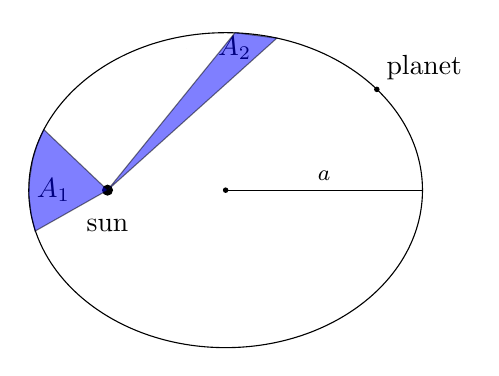
\begin{tikzpicture}
      \draw [rotate around={0:(1.5,0)}] (1.5,0) ellipse (2.5cm and 2cm);
%
      \fill (0,0) coordinate (O) circle (2pt) node[below =7pt] {sun};
      \fill (0,0) coordinate (O) circle (0pt) node[left =10pt] {$A_1$};
      \fill (1,1.8) coordinate (blah) circle (0pt) node[right =8pt] {$A_2$};
      %
      \coordinate (A1) at (1.62,2) ;%%
      \coordinate (A2) at (2.15,1.93);%%
      \coordinate (B1) at (-0.81,0.77);%%
      \coordinate (B2) at (-0.9,0.56);%%
      \coordinate (B3) at (-0.95,0.39);%%
      \coordinate (B4) at (-0.99,0.14);%%
      \coordinate (B5) at (-1,-0.05);%%
      \coordinate (B6) at (-0.97,-0.31);%%
      \coordinate (B7) at (-0.92,-0.52);%%
    %
%
      \coordinate (C1) at (3.25,-1.43);%%
      \coordinate (C2) at (3.51,-1.18);%%
%
      \coordinate (P) at (3.42,1.28) ;%%
      \fill (P) circle (1pt) node[above right] {planet};%
%
%
      \filldraw[fill=blue,opacity=0.5] (O) -- (A1) -- (A2) --cycle;%
      \filldraw[fill=blue,opacity=0.5] (O) -- (B1) -- (B2) -- (B3) -- (B4) -- (B5) -- (B6) -- (B7)
      --cycle;%
%

      \draw (1.5,0) coordinate (M) --node[above]{\footnotesize $a$}
      (4,0);%
      
      \fill (M) circle (1pt);
   \end{tikzpicture}
	\vspace*{-4pt}
	\end{center}


	\end{enumerate}

\end{theorem}



\begin{proof}[Proof of Kepler's First Law]
Inverse square law:
\[F(r) = -k/r^2 \implies F(u^{-1}) = -ku^2\]
Substituting into our orbital equation (6.6)
\[\frac{d^2u}{d\theta^2} + u = \frac{k}{mh^2u^2} ~(*)\]

This resembles \[m\frac{d^2x}{dt^2} + kx = F_0\]
The general solution to $(*)$ is $u = A\cos(\theta-\theta_0) + \dfrac{k}{mh^2}$;
 wlog take $\theta_0 = 0$ so
\[u(\theta) = A\cos(\theta) + \dfrac{k}{mh^2}\]
\begin{equation}\implies r(\theta) = \frac{(mh^2/k)}{1 + \frac{Amh^2}{k}\cos\theta}\end{equation}


This is the form of an ellipse in polar coordinates (see Problem 10, P.S. 1)
 
\[r(\theta) = \frac{l}{1 + e\cos\theta}\]
Where $l = \dfrac{mh^2}{k}$, $e = \dfrac{Amh^2}{k}$. \vspace*{150pt}

$e = [1-b^2/a^2]^{1/2}$,~$l = a(1-e^2)$ \end{proof}

We see that $E$ is related to $A$.
 
We can get the family of orbits by considering the energy; equation (6.5) gives
\[E = \frac{1}{2}m[\dot{r}^2 + r^2\dot{\theta}^2] + V(r)\]
 
 
 $F(r) =-kr^{-2} = -\dfrac{dV}{dr}$, so $ V(r) = -kr^{-1} \implies V(u^{-1}) = -ku$. 

Also $\dot{r} = -h\dfrac{du}{d\theta}$, and $r^2\dot{\theta}^2 = h^2r^{-2} = h^2u^2$. So the energy is
\[E = \frac{1}{2}mh^2\left[\left(\frac{du}{d\theta}\right)^2 + u^2\right]-ku\]
Using the fact $u(\theta) = A\cos(\theta) + \dfrac{k}{mh^2}$, $\dfrac{du}{d\theta} = -A\sin\theta$ and simplifying the trig we get
\[E = \frac{1}{2}mh^2A^2 - \frac{1}{2}\frac{k^2}{mh^2}\]
\[\implies A = \sqrt{\frac{2E}{mh^2} + \frac{k^2}{(mh^2)^2} }\]


From (6.9), the eccentricity of the orbit, $e = (1-b^2/a^2)^{1/2}$, is
\[e = \frac{Amh^2}{k} = \frac{mh^2}{k}\sqrt{\frac{2E}{mh^2} + \frac{k^2}{(mh^2)^2} } = \sqrt{1 + \frac{2Emh^2}{k^2}}\]
	

This parameter $e$ actually allows our solution $r(\theta)$ to describe a whole family of orbits. 
\begin{examples}
\begin{enumerate}
\item Bounded Trajectories
\begin{itemize}
\item $E = -k^2/2mh^2 \implies e = 0$ [Circle] 	
\item $E < 0 \implies 0 < e < 1$ [Ellipse]
\end{itemize}

\item Unbounded Trajectories
\begin{itemize}
\item $E = 0 \implies e = 1$ [Parabola]
\item $E > 0 \implies e > 1$ [Hyperbola]	
\end{itemize}

\end{enumerate}
	
\end{examples}

\subsektion{Effective Potential}
\lecturemarker{25}{22 Oct}
Consider the energy 
\[E = \frac{1}{2}m\dot{r}^2 + \frac{1}{2}mr^2\dot{\theta}^2 + V(r)\]

Since $h = r^2\dot{\theta},~ h^2 = r^4\dot{\theta}^2 \implies r^2\dot{\theta}^2 = h^2/r^2$
\[E = \frac{1}{2}m\dot{r}^2 + \frac{1}{2}\frac{mh^2}{r^2} + V(r)\]

\begin{definition}
The \emph{Effective Potential}, $V_{EFF} =\dfrac{1}{2}\dfrac{mh^2}{r^2} + V(r)$	
\end{definition}
\[\implies E = \frac{1}{2}m\dot{r}^2 + V_{EFF}\]
What we've done is written our energy in such a way that it looks like what we had with 1D motion! 
\[\begin{aligned}x &\longrightarrow r \\
V(x) &\longrightarrow V_{EFF}(r)
\end{aligned}
\]

\begin{definition} \emph{Turning points} occur when $V_{EFF} = E$. This tells us where $\frac{1}{2}m\dot{r}^2 = 0 \implies \dot{r} = 0$. This tells us about the boundedness of our orbit. 

\end{definition}
\pagebreak

\subsubsektion{Equilibria}
In 1D: $V'(x_0) = 0 \implies F(x_0) = 0$, where $x_0$ is the equilibrium point

If $\dot{x} = 0$ and $x = x_0$ at $t = 0$, then $m\ddot{x} = 0$ and $x = x_0~\forall t$

\[V_{EFF} =\dfrac{1}{2}\dfrac{mh^2}{r^2} + V(r)\]
\[\implies \frac{dV_{EFF}}{dr} = -mh^2r^{-3} + \underbrace{V'(r)}_{-F(r)}\]

Newton's 2nd Law's $\hat{r}$ component (equation (6.2))
\[m(\ddot{r} - r\dot{\theta}^2) = F(r)\]
\[\implies m\ddot{r} = F(r) + \frac{mh^2}{r^3} = \frac{dV_{EFF}}{dr}\]

Suppose that $V'_{EFF}(r_0) = 0$. If $r = r_0$ and $\dot{r} = 0$ at $t = 0$, then $m\ddot{r} = 0 \implies r = r_0~\forall t$. So we have a constant $r\implies $ Circular Trajectory

\subsubsektion{Stability}
$R = r-r_0$, $|R| << 1$, then the Taylor expansion about $r_0$:
\begin{equation}V_{EFF}(r) = V_{EFF}(r_0) + RV'_{EFF}(r_0) + \frac{1}{2}R^2V''_{EFF}(r_0) + \dots	
\end{equation}


Since at $r_0$, $V'_{EFF}(r_0) = 0$
\[V_{EFF}(r) = V_{EFF}(r_0) + \frac{1}{2}R^2V''_{EFF}(r_0)\]
Differentiating
\[V'_{EFF}(r) = RV''_{EFF}(r)\]

Using this in Newton's Second Law: 
\[m\ddot{r} = -RV''_{EFF}(r_0)\]
or 
\[m\ddot{R} + RV''_{EFF}(r_0)= 0\]

\begin{itemize}
\item If $V''_{EFF}(r_0)>0 \implies$ a minimum, so the circular orbit is stable.

\item If $V''_{EFF}(r_0) < 0 \implies$ a maximum, so the circular orbit is unstable. 
\end{itemize}~


\begin{example}
	$F(r) = -kr^{-2} ~(k > 0) \implies V(r) = -kr^{-1}$
	
	 \[\implies V_{EFF}(r) = -kr^{-1} + \frac{1}{2}mh^2r^{-2}\] 
	 \[\implies V'_{EFF}(r) = kr^{-2} - mh^2r^{-3}\]
	 
	 Setting this equal to zero 
	 \[r^{-3}(kr -mh^2) = 0\]
	 This is satisfied as $r \to \infty$ or at $r_0 = mh^2/k$
	 
	 \[V''_{EFF}(r) = -2kr^{-3} + 3mh^2r^{-4}\]
	 
	 So at the equilibria point
	 \[V''_{EFF}(mh^2/k) = \left(\frac{k}{mh^2}\right)^4(3mh^2 - 2k(mh^2/k)) = \left(\frac{k}{mh^2}\right)^4(mh^2)  > 0\]
	 This is a stable circular trajectory.
	 
	 \vspace*{150pt}
	 
\[ V'_{EFF}(\frac{mh^2}{k}) = -k\left(\frac{k}{mh^2}\right) + \frac{1}{2}mh^2\left(\frac{k^2}{(mh^2)^2}\right) = -\frac{k^2}{2mh^2}\] 

Thus \[E_{MIN} = -\frac{k^2}{2mh^2}.\]


We reach the same family of orbits as Example 6.10 by differing values of $E$:
\begin{enumerate}
\item Bounded Trajectories
\begin{itemize}
\item $E = E_{MIN} = -k^2/2mh^2 \implies r = \frac{mh^2}{k} \implies$ Circular Orbit
\item $E_{MIN} < E < 0 \implies $ two turning points $\implies$ Bounded Orbit [Ellipse]

\end{itemize}

\item Unbounded Trajectories when $E \geq 0$ since we have only a single turning point. In particular
\begin{itemize}
\item $E = 0 \implies $ Parabola
\item $E > 0 \implies $ Hyperbola
\end{itemize}

\end{enumerate}
\end{example}



		% Endomorhisms
%!TEX root = linear-algebra.tex
\stepcounter{lecture}
\setcounter{lecture}{7}


\sektion{Systems of Particles}
\lecturemarker{26}{22 Oct}

\begin{definition}
\begin{itemize}
\item N: Total number of particles
\item $\vec{r}_i$: Position of particle $i$
\item $\vec{v}_i$: Velocity of particle $i$
\item $\vec{F}_i$: Force on particle $i$
 \item $m_i$: Mass of particle $i$
\end{itemize}	
\end{definition}

\vspace*{60pt}

Consider the average motion of the system:

\begin{definition}
\emph{Centre of Mass}, $\vec{r}_{cm}$:
\[\vec{r}_{cm} = \frac{\sum_{i=1}^Nm_i\vec{r}_i}{\sum_{i=1}^Nm_i} =\frac{\sum_{i=1}^Nm_i\vec{r}_i}{M}  \]
Where $M = \sum_{i=1}^Nm_i$ is the \emph{total mass}. 	
\end{definition}

\subsubsektion{Momentum}

The total momentum $\vec{p}$ is
\[\begin{aligned}\vec{p} = \sum_i\vec{p}_i = \sum_im_i\vec{v}_i &= \sum_i m_i\frac{d\vec{r}_i}{dt} \\
 &= \frac{d}{dt}(\sum_i m_i\vec{r}_i) \\
 &= \frac{d}{dt}(M\vec{r}_{cm}) \\
 &= M\frac{d\vec{r}_{cm}}{dt} = M\vec{v}_{cm}
\end{aligned}
\]

Where $\vec{v}_{cm}$ is the velocity of the centre of mass.


\[\vec{F}_i = \vec{F}_i^{EXT} + \sum_{j=1}^N \vec{F}_{ij}\]
where $\vec{F}_i^{EXT}$ is the external forces on particle $i$, $\vec{F}_{ij}$ is the force on $i$ due to $j$
\begin{example}
\vspace*{45pt}

Here $\vec{F}_{gi}$(Force due to gravity on $i$) is the only external force on $i \implies \vec{F}_i^{EXT} = \vec{F}_{gi}$
	
\end{example}

Note that
\begin{enumerate}
\item $\vec{F}_{ii} = \vec{0}$
\item $\vec{F}_{ij} = -\vec{F}_{ji}$ By Newton's Third Law
\end{enumerate}

\begin{theorem}[Newton's Second Law for a System]
The external force is equal to the rate of change of momentum of the centre of mass
	\[M\frac{d\vec{v}_{cm}}{dt} = \vec{F}^{EXT}\]
	Where the total external force on the system $\vec{F}^{EXT} = \sum_i\vec{F}_i^{EXT}$.
\end{theorem}
\begin{proof}

For particle $i$, \[\dfrac{d\vec{p}_i}{dt} = \vec{F}_i = \vec{F}_i^{EXT} + \sum_{j=1}^N\vec{F}_{ij}\] 
\[\implies \sum_i \dfrac{d\vec{p}_i}{dt} = \sum_i\vec{F}_i = \sum_i\vec{F}_i^{EXT} + \sum_i\sum_j\vec{F}_{ij} \]
Due to Newton's Third Law $\sum_i\sum_j\vec{F}_{ij} = \vec{0}$. We are then left with 
\[\begin{aligned}\sum_i\dfrac{d\vec{p}_i}{dt} &= \sum_i\vec{F}_i^{EXT}\\
\implies \dfrac{d}{dt}(\sum_i \vec{p}_i) &= \vec{F}^{EXT}\end{aligned}
\]
\[\implies M\frac{d\vec{v}_{cm}}{dt} = \vec{F}^{EXT}\qedhere\]
\end{proof}

\begin{enumerate}
\item If there is no external forces then 
\[M \frac{d\vec{v}_{cm}}{dt} = 0 = \frac{d\vec{p}}{dt}\]
(The conservation of momentum)
\item	If there are external forces then the centre of mass moves as though it were a point particle of mass $m$ subject to force $\vec{F}^{EXT}$
\end{enumerate}


\subsektion{Two Body Problems}
\vspace*{50pt}

$\vec{F}_1 = m_1g \hat{i} + \vec{F}_{12}$

$\vec{F}_2 = m_2g \hat{i} + \vec{F}_{21}$

The total external force:
\[\vec{F}^{EXT} = m_1g\hat{i} + m_2g\hat{i} = Mg\hat{i} ~(M = m_1 + m+2)\]
Thus
\[M\frac{d\vec{v}_{cm}}{dt} = Mg\hat{i} \implies \frac{d\vec{v}_{cm}}{dt} = g\hat{i}\]

For two body problems this is half of the information.

\begin{equation}
m_1\frac{d^2\vec{r}_1}{dt^2} = \vec{F}_1^{EXT} + \vec{F}_{12}	
\end{equation}

\begin{equation}
m_2\frac{d^2\vec{r}_2}{dt^2} = \vec{F}_2^{EXT} + \vec{F}_{21}	
\end{equation}
Calling $\dfrac{m_1\vec{r}_1 + m_2\vec{r}_2}{m_1 + m_2}$, and adding the equations
\setlength{\jot}{10pt}
\[\begin{aligned}m_1\frac{d^2\vec{r}_1}{dt^2} + m_2\frac{d^2\vec{r}_2}{dt^2} &= \vec{F}_1^{EXT} + \vec{F}_{2}^{EXT}\\
M \frac{d}{dt}\left(\frac{m_1\vec{v}_1 + m_2\vec{v}_2}{M}\right) &=  \vec{F}_1^{EXT} + \vec{F}_{2}^{EXT}\\
M\frac{d\vec{v}_{cm}}{dt} &=  \vec{F}_1^{EXT} + \vec{F}_{2}^{EXT}
\end{aligned}\]

\lecturemarker{27}{22 Oct}
Consider: $m_2 \times (7.4) - m_1\times(7.3)$
\[m_1m_2\frac{d^2}{dt^2}(\vec{r}_1-\vec{r}_2) = m_2\vec{F}_1^{EXT} + m_1\vec{F}_2^{EXT} + m_2\vec{F}_{12} - m_1\vec{F}_{21}\]
Call $\vec{r}_{12} = (\vec{r}_1 - \vec{r}_2)$. Since $\vec{F}_{12} = -\vec{F}_{21}$
\[m_1m_2\frac{d^2\vec{r}_{12}}{dt^2} = m_2\vec{F}_1^{EXT} + m_1\vec{F}_2^{EXT} + (m_1 + m_2)\vec{F}_{12}\]
Divide through by $M$
\[\frac{m_1m_2}{M}\frac{d^2\vec{r}_{12}}{dt^2} = \frac{m_2\vec{F}_1^{EXT} + m_1\vec{F}_2^{EXT}}{M} + \vec{F}_{12}\]
\begin{definition} Introduce $\mu = \dfrac{m_1m_2}{M}$, the \emph{reduced mass}.
\end{definition}
Then for our two body system we have:
\begin{equation}
M\frac{d\vec{v}_{cm}}{dt} =  \vec{F}_1^{EXT} + \vec{F}_{2}^{EXT}
\end{equation}
\begin{equation}
\mu\frac{d^2\vec{r}_{12}}{dt^2} = \frac{m_2\vec{F}_1^{EXT} + m_1\vec{F}_2^{EXT}}{M} + \vec{F}_{12}
\end{equation}~

If $\vec{F}_1^{EXT} = \vec{F}^{EXT}_2 = 0$, then $M\dfrac{d\vec{v}_{cm}}{dt} = 0$, and $\mu\dfrac{d^2\vec{r}_{12}}{dt^2}  = \vec{F}_{12}$.

If $\vec{F}_1^{EXT} = -m_1g\hat{j}$ and $\vec{F}^{EXT}_2 = -m_2g\hat{j}0$, then $M\dfrac{d\vec{v}_{cm}}{dt} = -Mg\hat{j}$, and $\mu\dfrac{d^2\vec{r}_{12}}{dt^2}  = \vec{F}_{12}$.



\begin{example}[Spring]
\vspace*{50pt}

Speing has a spring constant $k$ and equilibrium lnegth $l$. 
\[\vec{F}_{12} = -k(x_1 - x_2 - l)\hat{i}\]

Initially $x_1(0) = k,~ \dot{x}_1 = v_0$. $x_2(0) = \dot{x}_2(0) = 0$.

$\vec{F}_{12}$ is the only force in the $\hat{i}$ direction. No external forces in the $\hat{i}$ direction. 
\[\implies M\ddot{x}_{cm} = 0 \implies \dot{x}_{cm} = C\]
We can find $C$ using the conservation of momentum
\[\vec{p} = m\dot{x}_1 + m\dot{x}_2 = M\dot{x}_{cm}\]
At $t = 0, \dot{x}_1 = v_0$ and $\dot{x}_2 = 0$. Then $p = mv_0$. Since $M = 2m$:
\[\dot{x}_{cm} = v_0/2\]

For $x_{12} = x_1 - x_2$
\[\mu = \frac{m_1m_2}{m_1 + m_2} = \frac{m^2}{2m} = \frac{m}{2}\]
\[\vec{F}_{12} = -k(x_1 - x_2 - l) = -k(x_{12} - l)\]

Using the equation for $\vec{r}_{12}$
\[\begin{aligned}\mu\ddot{x}_{12} &= \vec{F}_{12}\\
\frac{m}{2}\ddot{x}_{12} &= -k(x_{12} - l)\\
\ddot{x}_{12} + \frac{2k}{m}x_{12} &= \frac{2kl}{m}	
\end{aligned}
\]

The general solution is 
\[x_{12} = A\cos\omega t + B\sin\omega t + l\]
where $\omega^2 = \frac{2k}{m}$. 

From our initial conditions $x_{12}(0) = x_1(0) - x_2(0) = l$ and $\dot{x}_{12} = v_0$. 
\[\implies A = 0,~B = v_0/\omega\]Thus
\[x_{12} = \frac{v_0}{\omega}\sin\omega t + l\]
\[\dot{x}_{12} = v_0\cos\omega t\]

We can show that (in general)
\[\vec{r}_1 = \vec{r}_{cm} + \vec{m_2}{M}\vec{r}_{12}\]
\[\vec{r}_2 = \vec{r}_{cm} + \vec{m_1}{M}\vec{r}_{12}\]

Thus
\[x_1 = x_{cm} + \frac{1}{2}x_{12}\]
\[\dot{x}_1 = \dot{x}_{cm} + \frac{1}{2}\dot{x}_{12} = \frac{v_0}{2} + \frac{1}{2}v_0\cos\omega t = \frac{v_0}{2}(1+\cos\omega t)\]
Similarly 
\[\dot{x}_2 =  \frac{v_0}{2}(1 - \cos\omega t)\]
This is a push-me-pull-you system.
\end{example}

\emph{What about more than two particles?}\\

\begin{definition}[Centre of Mass Coordinates]
\[\vec{R}_i = \vec{r}_i - \vec{r}_{cm}\]	
This is the position of particle $i$ relative to the position of the centre of mass
\end{definition}

\[\sum_im_i\vec{R}_i = \underbrace{\sum_im_i\vec{r}_i}_{M\vec{r}_{cm}}- \vec{r}_{cm}\underbrace{\sum_im_i}_{M} = 0\]








\subsubsektion{Kinetic Energy}
\lecturemarker{28}{22 Oct}
\[T = \sum_i \frac{1}{2}m_iv_i^2\]
We can write $\vec{v}_i = \vec{v}_{cm} + \dfrac{d\vec{R}_i}{dt},~\vec{u}_i = \dfrac{d\vec{R}_i}{dt}$, so $\vec{v}_i = \vec{v}_{cm} + \vec{u}_i$

\[\begin{aligned}T &= \sum_i \frac{1}{2}m_i(\vec{v}_{cm}+\vec{u}_i) \cdot(\vec{v}_{cm}+\vec{u}_i)\\
&= \sum_i \frac{1}{2}[v_{cm}^2 + 2\vec{u}_i\cdot\vec{v}_{cm} + u_i^2\\
&= 	\frac{1}{2}v_{cm}^2\sum_i m_i + \vec{v}_{cm}\cdot\sum_im_i\vec{u}_i + \frac{1}{2}\sum_im_iu_i^2\\
&= \frac{1}{2}Mv_{cm}^2 + \frac{1}{2}\sum_im_iu_i^2 + \vec{v}_{cm}\cdot\sum_im_i\vec{u}_i
\end{aligned}
\]
Consider $\sum_i m_i\vec{u}_i = \sum_im_i\dfrac{d\vec{R}_i}{dt} = \dfrac{d}{dt}(\sum_i m_i\vec{R}_i) = 0$. Then 
\begin{equation}\boxed{T = \frac{1}{2}Mv_{cm}^2 + \sum_i\frac{1}{2}m_iu_i^2}\end{equation}

\subsektion{Angular Momentum}

\[\vec{J} = \vec{r} \times \vec{p} = \vec{r} \times m\vec{v}\]
For central forces where the motion was restricted to a plane $\vec{J} = mh\hat{k} =$ constant vector. 

\emph{What causes $\vec{J}$ to change?}

\[\begin{aligned}\frac{d\vec{J}}{dt} &= \frac{d\vec{r}}{dt} \times m \vec{v} + \vec{r}\times \frac{d\vec{v}}{dt}\\ &= m\cancelto{0}{[\vec{v} \times \vec{v}]} + \vec{r} \times \vec{F} = \vec{\tau}\end{aligned}
\]

\begin{definition}
$\vec{\tau} = \vec{r} \times \vec{F}$ is the \emph{Torque} or the \emph{Moment}. 
\vspace*{50pt}
\begin{itemize}
\item $\vec{\tau}$ is in the direction out of the screen
\item $|\vec{\tau}| = |\vec{F}||\vec{r}|\sin\phi$ 	
\end{itemize}
\end{definition}

For central forces 
\vspace*{50pt}

Since $\phi = 0 \implies \vec{\tau} = 0$. 

For a system, the total angular momentum
\[\vec{J} = \sum_{i}\vec{J}_i = \sum_i\vec{r}_i \times m_i \vec{v}_i\]
\[\implies \vec{\tau} = \frac{d\vec{J}}{dt} = \sum_i\dfrac{d\vec{J}_i}{dt} = \sum_i\vec{r}_i\times\vec{F}_i\]
Write $\vec{F}_i = \vec{F}_i^{EXT} + \sum_j\vec{F}_{ij}$. Then we have
\begin{equation} \vec{\tau} \frac{d\vec{J}}{dt} = \sum_i\vec{r}_i\times\vec{F}_i^{EXT} + \sum_i\sum_j\vec{r}_i\times\vec{F}_{ij}\end{equation}


\begin{theorem}[Conservation of Angular Momentum for a System]
If there is no net torque, the angular momentum is conserved.
\end{theorem}

\begin{proof}[Proof (for two body system)]

Suppose we have two particles. Then the double sum is 
\[\vec{r}_1 \times\vec{F}_{12} +\vec{r}_2 \times\vec{F}_{21} \]

By Newton's Third Law $\vec{F}_{12} = -\vec{F}_{21}$. Thus
\[\vec{r}_1 \times\vec{F}_{12} +\vec{r}_2 \times\vec{F}_{21} = (\vec{r}_1 - \vec{r}_2) \times \vec{F}_{12}\]

If $\vec{F}_{12}$ is parallel to $\vec{r}_1 - \vec{r}_2$, then $(\vec{r}_1 - \vec{r}_2) \times \vec{F}_{12} = 0$. 

This is the case if $\vec{F}_{12}$ is a central force, i.e. no torque. 

Thus if $\vec{F}_{ij}$ is a central force for all $i$ and $j$. Then 
\[\sum_i\sum_j \vec{r}_i \times \vec{F}_{ij} = \vec{0}\]

Then 
\[\frac{d\vec{J}}{dt} = \sum_i\vec{r}_i \times \vec{F}_i^{EXT} = \vec{\tau}^{EXT}\]
where $\vec{\tau}^{EXT}$ is the total external torque on the system.

So if $\vec{\tau}^{EXT} = \vec{0}$ then $\dfrac{d\vec{J}}{dt} = \vec{0}$, hence the angular momentum is conserved.
\end{proof}

\begin{example}
\vspace*{50pt}

Each particle has mass $m$. Each mass has velocity $\vec{v}_i = \vec{\omega} \times \vec{r}_i$, with $\vec{\omega} = \omega\hat{k}$	

The angular momentum of particle $i$ is:
\[\vec{J}_i = \vec{r}_i \times m_i\vec{v}_i = m[\vec{r}_i \times (\vec{\omega} \times \vec{r}_i)]\]

Recall that $\vec{A} \times (\vec{B} \times \vec{C}) = (\vec{A}\cdot\vec{C})\vec{B} - (\vec{A}\cdot\vec{B})\vec{C}$
\[\vec{r}_i \times (\vec{\omega} \times \vec{r}_i) = (\vec{r}_i \cdot \vec{r}_i)\vec{\omega} - \cancelto{0}{(\vec{r}_i \cdot \vec{\omega})}\vec{r}_i = r^2\omega\hat{k}\]

Thus 
\[\vec{J}_i = mr^2\omega\hat{k}\]
\[\implies \vec{J} = \sum_i \vec{J}_i = 4mr^2\omega\hat{k} = 2ml^2\omega\hat{k}\]

Suppose that 
\vspace*{50pt}

$\vec{v}_i = \vec{\omega} \times \vec{r}_i \longrightarrow \vec{v}_i = \vec{\Omega} \times\vec{r}_i$. What's $\vec{\Omega}$?

Single the configuration changed to to internal, central forces, $\dfrac{d\vec{J}}{dt} = 0$

For our new configuration
\[\vec{J}_i = 2m[\vec{r}_i \times (\vec{\Omega} \times \vec{r}_i)] = 2mr_i^2\Omega\hat{k} = \frac{ml^2\Omega}{2}\hat{k}\]
The total angular momentum
\[\vec{J} = 2\vec{J}_i = ml^2\Omega\hat{k}\]

Since $\dfrac{d\vec{J}}{dt} = 0 \implies \vec{J}_{before} = \vec{J}_{after}$

\[\implies 2ml^2\omega\hat{k}= ml^2\Omega\hat{k}\]
\[\implies \Omega = 2\omega\]

The angular speed doubles as a result of the change. 
\end{example}~\\

\subsubsektion{Centre of Mass Coordinates}
\lecturemarker{29}{22 Oct}

\[\vec{r}_i = \vec{r}_{cm} + \vec{R}_i\]
\[\vec{v}_i = \vec{v}_{cm} + \vec{u}_i,~\left(\vec{u}_i = \frac{d\vec{R}_i}{dt}\right)\]
Thus
\[\begin{aligned}
\vec{J} &= \sum_i (\vec{r}_{cm} + \vec{R}_i) \times m_i(\vec{v}_{cm} + \vec{u}_i)\\
&= \sum_i \vec{r}_{cm} \times m_i\vec{v}_{cm} + \sum_i \vec{r}_{cm} \times m_i\vec{u}_i + \sum_i \vec{R}_i \times m_i\vec{v}_{cm} + \sum_i \vec{R}_i \times m_i\vec{u}_i\\
&= \vec{r}_{cm}\times \vec{v}_{cm}(\sum_i m_i) + \vec{r}_{cm} \times (\sum_i m_i\vec{u}_i) + (\sum_im_iR_i)\times\vec{v}_{cm} + \sum_iR_i\times m_i\vec{u}_i
\end{aligned}
\]

We know that $\sum_i m_i = M$, $\sum_i m_i\vec{R}_i = \sum_i m_i \vec{u}_i = 0$. Thus
\[\vec{J} = \vec{r}_{cm} \times M\vec{v}_{cm} + \sum_i\vec{R}_i\times m_i\vec{u}_i\]

%Contribution to centre of mass, and motion relative to centre of mass.
Call $\vec{J}_{cm} = \sum_i \vec{R}_i \times m_i\vec{u}_i$

Recall that 
\[\frac{d\vec{J}}{dt} = \sum_i \vec{r}_i \times \vec{F}_i^{EXT} (= \vec{\tau}^{EXT})\]
Since $\vec{r}_i = \vec{r}_{cm} + \vec{R}_i$
\[\begin{aligned} \frac{d\vec{J}}{dt} &= = \sum_i \vec{r}_{cm} \times \vec{F}_i^{EXT}\\
&= \vec{r}_{cm} \times \vec{F}^{EXT} + \sum_i\vec{R}_i\times\vec{F}_i^{EXT}
\end{aligned}
\]

We can show (P.S. 4 Problem 9)
\[\frac{d\vec{J}_{cm}}{dt} = \sum_i\vec{R}_i\times\vec{F}_i^{EXT}\]
Call
\[\vec{\tau}_{cm}^{EXT} = \sum_i\vec{R}_i \times \vec{F}_i^{EXT}\]

\subsubsektion{Complete Picture}
\begin{enumerate}
\item Momentum: \[\vec{p} = M\vec{v}_{cm}\]
\[\frac{d\vec{p}}{dt} =  M\frac{d\vec{v}_{cm}}{dt} = \vec{F}^{EXT}\]
\item Angular Momentum: \[\vec{J} = \vec{r}_{cm} \times M\vec{v}_{cm} + \vec{J}_{cm}\]
\[\vec{J}_{cm} = \sum_i\vec{R}_i \times m_i\vec{u}_i\]
\[\frac{d\vec{J}}{dt} = \vec{r}_{cm} \times \vec{F}^{EXT} + \vec{\tau}_{cm}^{EXT}\]
\end{enumerate}



















		% Endomorhisms
%!TEX root = linear-algebra.tex
\stepcounter{lecture}
\setcounter{lecture}{8}


\sektion{Rigid Body Motion}
\begin{definition}
\emph{Rigid Body Motion} occurs when 
\[\frac{d|\vec{r}_- \vec{r}_j|}{dt} = 0,~ \forall i,j\]
For such a system
\[\vec{v}_i = \vec{v}_{cm} + \underbrace{\vec{\omega}\times\vec{R}_i}_{\vec{u}_i}\]	
Where $\vec{\omega}$ is the \emph{angular velocity of the rigid body}.

We can also write 
\[\vec{v}_i = \vec{V} + \vec{\omega}\times\vec{r}_i\]
where 
$\vec{V} = \vec{v}_{cm} - \vec{\omega}\times\vec{r}_{cm}$
\end{definition}

To determine the motion of the system we'll need to find $\vec{v}_{cm}$ and $\vec{\omega}$. For $\vec{v}_{cm}$ we already have this!
\begin{equation}M\frac{d\vec{v}_{cm}}{dt} = \vec{F}^{EXT}\end{equation}

What about $\vec{\omega}$?
\[\vec{J}_{cm} = \sum_i\vec{R}_i\times m_i\vec{u}_i\]

For a rigid body $\vec{u}_i = \vec{\omega}\times\vec{R}_i$
\[\vec{J}_{cm} = \sum_i\vec{R}_i \times m_i(\vec{\omega}\times\vec{R})i) = \sum_i m_i(\vec{R}_i\times(\vec{\omega}\times\vec{R}_i))\]

From the identity for the triple vector product, we have
\[\vec{J}_{cm} = \sum_im_i[R_i^2\vec{\omega} - (\vec{\omega}\cdot\vec{R}_i)\vec{R}_i]\]

Consider only planar motion: we have $\vec{\omega} = \omega\hat{k}$, and $\vec{R}_i = X_i\hat{i} + Y_i\hat{j}$. Thus 
\[\vec{\omega}\cdot\vec{R}_i = 0,~\forall i\]

As a result:
\begin{equation}
\vec{J}_{cm} = \underbrace{(\sum_im_iR_i^2)}_{I_{cm}}\vec{\omega}	
\end{equation}

\begin{definition}
$I_{cm}$ is the \emph{moment of inertia} about the centre of mass.	
\end{definition}

For this Rigid Body Motion $\dfrac{d|R_i|}{dt} = 0$. This means that $I_{cm}$ is constant.

Consider
\[\frac{d\vec{J}_{cm}}{dt} = I_{cm}\frac{d\vec{\omega}}{dt} = \vec{\tau}_{cm}^{EXT} = \sum_i\vec{R}_i\times\vec{F}_i^{EXT}\]

For a rigid body undergoing planar motion:
\begin{equation}M\frac{d\vec{v}_{cm}}{dt} = \vec{F}^{EXT}\end{equation}
\begin{equation}I_{cm}\frac{d{\omega}}{dt} = {\tau}_{cm}^{EXT}\end{equation}
 (Scalar Equation since all in $\hat{k}$)
 
\subsektion{Kinetic Energy}~
\[T = \frac{1}{2}M\vec{v}_{cm}^2 + \frac{1}{2}\sum_im_i\vec{u}_i^2\]
$\vec{u}_i = \vec{\omega} \times \vec{R}_i$, $u_i^ 2 = (\vec{\omega}\times\vec{R}_i) \cdot (\vec{\omega}\times\vec{R}_i)$

For planar motion $|\vec{\omega}\times\vec{R}_i| = |\vec{\omega}||\vec{R}_i| \implies u_i^2 = \omega^2R_i^2$
\[\begin{aligned}T &= \frac{1}{2}M\vec{v}_{cm}^2 + \frac{1}{2}\left(\sum_im_i{R}_i^2\right)\omega^2\\
\implies 	T &= \frac{1}{2}M\vec{v}_{cm}^2 + \frac{1}{2}I_{cm}\omega^2
\end{aligned}
\]
\lecturemarker{30}{22 Oct}
\begin{definition}
The continuous case:
\[M = \sum_i m_i = \int_B \,dm\]
\[\vec{r}_{cm} = \frac{\sum_i m_i\vec{r}_i}{M} = \frac{\int_B\vec{r}\,dm}{M}\]
\[I_{cm} = \sum_i m_iR_i^2 =  \int_B R^2\,dm\]
Equations of motion remain the same.
\end{definition}~

\begin{example}[Uniform Rod]
	\vspace*{50pt}
\end{example}



\subsektion{* Parallel Axis Theorem *}
\lecturemarker{31}{22 Oct}

(Non-examinable in 2015)
\begin{theorem}[Parallel Axis Theorem]
For an axis, $P$, parallel to the centre of mass	\[I_P = I_{CM} + Mr^2_{CM}\]
\end{theorem}
\begin{proof}
\[\begin{aligned}I_P = \sum_{i} m_ir_i^2 &= \sum_i m_i(\vec{r}_{CM} + \vec{R}_i)^2\\
&= \sum_i m_i r_{CM}^2 + 2	
\end{aligned}
\]
\end{proof}

\begin{example}[Physical Pendulum]
	Blah
\end{example}






  \begin{center}
  \textsf{\textbf{- End of Mechanics -}}	
  \end{center}
  
  



		% Endomorhisms


\end{document}